\section{Results}
\label{sec:results}

\subsection{Gold evidence improves aggregate accuracy}
\label{sec:rq1}
Table~\ref{tab:accuracy} answers RQ1.
On the same 10{,}000 claims, designated gold evidence raises GPT-5.4 accuracy from 88.69\% to 96.04\% ($+7.35$~pp) and GPT-5.4-mini from 84.67\% to 95.54\% ($+10.87$~pp).
Paired McNemar tests are large (GPT-5.4 $\chi^2=558.3$, $p\approx 2\times 10^{-123}$; mini $\chi^2=849.1$, $p\approx 10^{-186}$).
Figure~\ref{fig:transitions} shows the four-way transition structure behind those averages.
Evidence also increases cross-model prediction agreement, from 89.3\% ($\kappa=0.786$) without evidence to 97.2\% ($\kappa=0.944$) with evidence.

\begin{figure}[t]
\centering
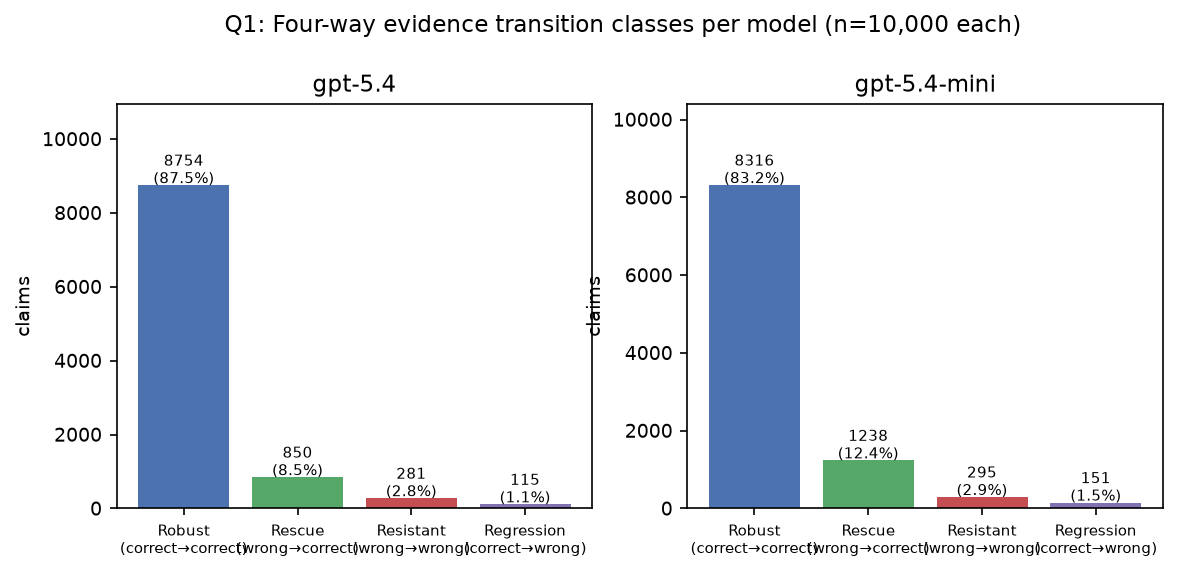
\includegraphics[width=0.92\linewidth]{../analysis_v2/figures/fig1_transition_matrices.png}
\caption{Paired transition matrices for GPT-5.4 and GPT-5.4-mini. Off-diagonal cells are rescues (wrong$\rightarrow$correct) and regressions (correct$\rightarrow$wrong).}
\label{fig:transitions}
\end{figure}

\subsection{Evidence can induce correct-to-wrong regressions}
\label{sec:rq2}
The same paired design produces 115 GPT-5.4 regressions (1.15\%, bootstrap 95\% CI $[0.95,1.36]$) and 151 mini regressions (1.51\%, CI $[1.28,1.75]$).
Rescues are more common: 850 (8.5\%) and 1{,}238 (12.4\%).
Among claim-only errors, evidence corrects 75.2\% (GPT-5.4) and 80.8\% (mini).

Unique-claim counts, not model-observations, are the regression cohort for later adjudication: 226 claims regress for at least one model, 40 for both, and 186 for exactly one (75 GPT-5.4-only, 111 mini-only).
A paired McNemar test on discordant claims finds a modest model difference in regression incidence (115 vs.\ 151, $\chi^2=6.59$, $p=0.010$).
87.3\% of claims share the same transition class across models.
RQ2's answer is therefore: regressions are real, rare relative to 10{,}000 claims, only partly shared, and large enough to study as a structured minority.
These behavioral results come from the original 40{,}000 predictions and are unaffected by the adjudication audit; they are observed outcomes of the original prompts, not evidence of repeat-run stability.

\subsection{Characteristics of evidence-induced regressions}
\label{sec:rq3-nli}
Regressions are not a random slice of the sample.
A local NLI diagnostic (nli-deberta-v3-small) disagrees with the FEVER label on 74.8\% of GPT-5.4 regressions and 76.8\% of mini regressions, against 22.6\% of GPT-5.4 robust successes (Figure~\ref{fig:nli}).
Resistant failures look similar (75.8\%).
A second, architecturally different NLI model reproduces the same ordering.
The 2{,}462 claims flagged as weakly warranted also have lower claim-only GPT-5.4 accuracy (81.0\% vs.\ 88.69\%), so the NLI signal marks hard items rather than a quirk of one evidence-condition model.

\begin{figure}[t]
\centering
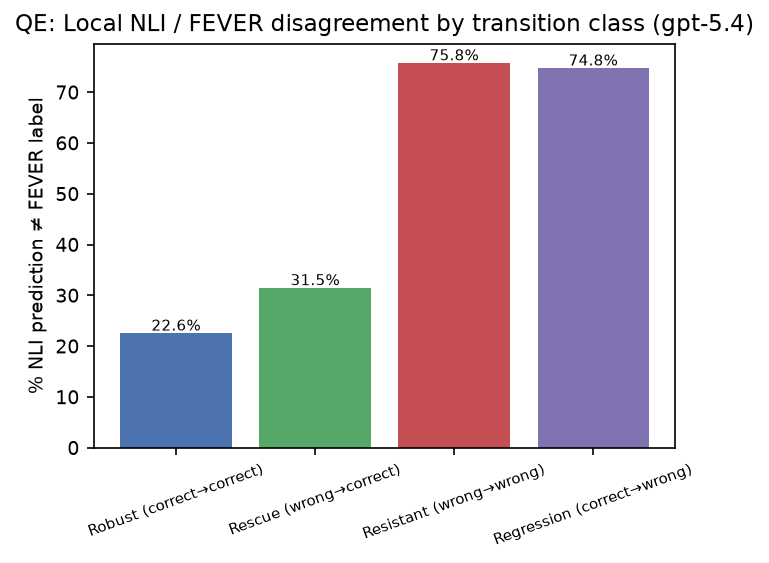
\includegraphics[width=0.88\linewidth]{../analysis_v2/figures/fig6_nli_disagreement.png}
\caption{Local NLI disagreement with the FEVER label by GPT-5.4 transition class. The NLI models are diagnostics, not a relabeling of FEVER.}
\label{fig:nli}
\end{figure}

Label asymmetry is model-dependent.
GPT-5.4 regressions concentrate on Supported claims (88 vs.\ 27 Refuted, $p=1.8\times 10^{-8}$); mini shows no such split (74 vs.\ 77, $p=0.87$).
Surface features (length, overlap, evidence-set size) only weakly separate regressions.
Predictive models that include NLI features do better than surface-only models, but rare-class PR-AUC remains low.
We treat this block as characterization; it does not depend on the adjudication stage that was corrected.

\subsection{Adjudication outcomes on repaired evidence}
\label{sec:rq3-adjudication}
Table~\ref{tab:diagnostic} and Figure~\ref{fig:categories} answer RQ3 for the 226 regressions.
Values in this and the next subsection use the accepted Stage~C outputs; the first-valid sensitivity selection is given where it differs (Section~\ref{sec:correction}).
The largest Grok categories are sentence-only gold agreement (77; 34.1\%, Wilson 95\% CI 28.2--40.5) and final nondecisiveness (71; 31.4\%, 25.7--37.7), whose intervals overlap.
Decisive verdicts that disagree with FEVER form the third group (44; 19.5\%, 14.8--25.1).
Title, structured and additional-evidence gold agreement together cover 29 claims (12.8\%), and five claims follow a nonmonotonic path.
Among regressions with a decisive Stage~C consensus, the Grok verdict agrees with FEVER on 111 of 155 (71.6\%).

\begin{figure}[t]
\centering
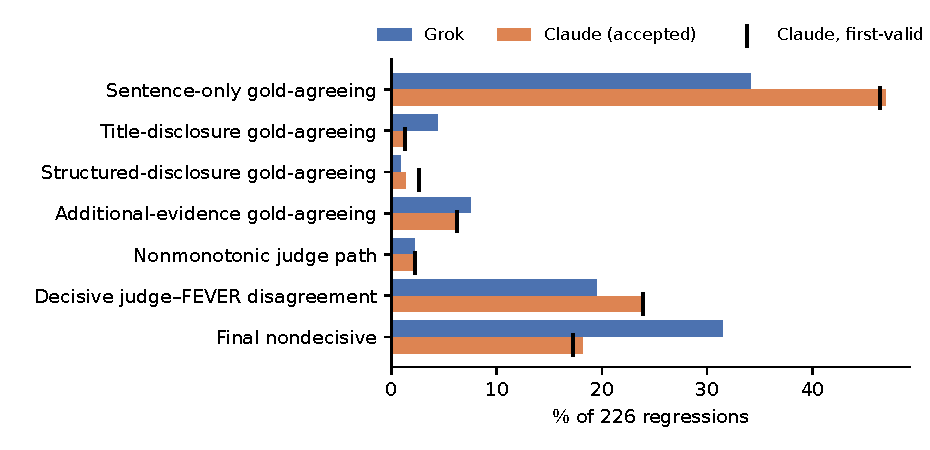
\includegraphics[width=0.95\linewidth]{figures/fig_categories.pdf}
\caption{Adjudication outcome categories for the 226 unique regressions on repaired Stage~C inputs, by adjudicating family. Bars use the accepted outputs; black ticks mark Claude under the first-valid sensitivity selection. Grok values are identical under both selections.}
\label{fig:categories}
\end{figure}

Progressive disclosure changes a minority of verdicts (Table~\ref{tab:stage}, Figure~\ref{fig:stage}).
Titles make 16 of the 103 Stage~A-nondecisive regressions decisive, and Stage~C makes 27 of the 95 Stage~B-nondecisive regressions decisive.
No decisive consensus is reversed by titles or by Stage~C.
Because Stage~C adds alternative sentence text for 41 regressions, Stage~C-associated changes cannot be attributed to representation alone; the 17 additional-evidence cases are separated from the two structure-only cases for that reason.

Shared regressions remain nondecisive more often than model-specific ones (Table~\ref{tab:shared}): 45.0\% versus 28.5\% under Grok (odds ratio 2.05, $p_{\mathrm{BH}}=0.059$).

The RQ3 answer is a mixture of FEVER-agreeing, FEVER-disagreeing and nondecisive outcomes, with no single dominant category under Grok.
These outcomes do not show why GPT changed its answer, and the decisive disagreements are not evidence that FEVER is wrong.

\subsection{Cross-family comparison}
\label{sec:rq4}
The Claude panel judges the same 226 regressions (1{,}130 new Stage~C judgments, paired with its 2{,}260 retained Stage~A/B judgments).
Claude assigns more regressions to sentence-only gold agreement (106, 46.9\%, CI 40.5--53.4; first-valid 105; $+12.8$ and $+12.4$~pp versus Grok, $p_{\mathrm{BH}}\le 2.1\times 10^{-6}$) and fewer to final nondecisiveness (41, 18.1\%, CI 13.7--23.7; first-valid 39; $-13.3$ and $-14.2$~pp, $p_{\mathrm{BH}}\le 9.1\times 10^{-8}$).
Decisive judge--FEVER disagreement is somewhat more common under Claude (54 versus 44; $+4.4$~pp, $p_{\mathrm{BH}}=0.015$).
Among decisive Stage~C consensus verdicts, FEVER agreement is similar across families (Claude 131/185, 70.8\%; Grok 111/155, 71.6\%).

Claude is more decisive at every stage (Table~\ref{tab:stage}, Figure~\ref{fig:stage}): nondecisive rates are 29.2\%, 28.3\% and 18.1\% (first-valid 17.3\%) versus Grok's 45.6\%, 42.0\% and 31.4\%.
Titles resolve 9 of Claude's 66 Stage~A-nondecisive regressions and Stage~C resolves 24 of its 64 Stage~B-nondecisive regressions (first-valid 27).
Title and Stage~C resolution rates do not differ significantly between families, and neither family reverses a decisive consensus.

\begin{figure}[t]
\centering
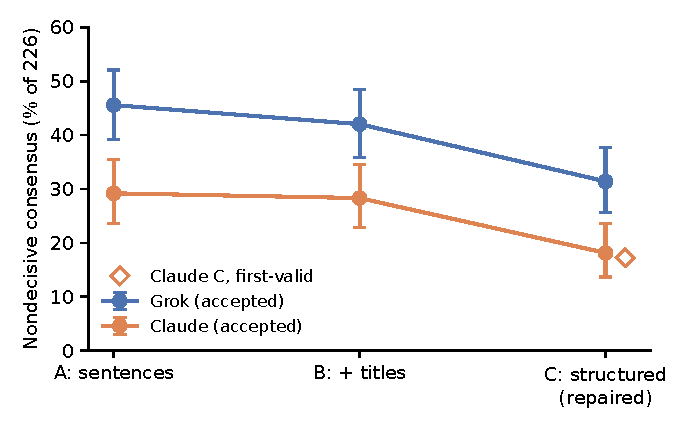
\includegraphics[width=0.62\linewidth]{figures/fig_stage_nondecisive.pdf}
\caption{Nondecisive (Ambiguous or Unresolved) five-judge consensus on the 226 regressions at each disclosure stage, with Wilson 95\% intervals. Stages~A and~B are retained historical judgments on unchanged inputs; Stage~C is new judgments on repaired inputs. The open diamond is Claude Stage~C under the first-valid sensitivity selection.}
\label{fig:stage}
\end{figure}
Under Claude, shared regressions are also more often nondecisive than model-specific ones (35.0\% versus 14.5\%; odds ratio 3.17, $p_{\mathrm{BH}}=0.011$; first-valid 3.47, $p_{\mathrm{BH}}=0.005$).

Exact per-claim category agreement is 172/226 (76.1\%, Wilson 70.1--81.2; $\kappa=0.673$) for the accepted selection and 168/226 (74.3\%, 68.3--79.6; $\kappa=0.651$) for first-valid.
The first-valid figure coincides numerically with the historical 74.3\%, which measured a different, withdrawn taxonomy on defective inputs; the two are not comparable.

\paragraph{Selection sensitivity.}
Substituting the first valid outputs for the accepted ones changes Stage~C consensus for six of the 226 Claude claims and for one of the 1{,}060 Grok claims (a rescue-cohort claim, so no Grok regression result changes).
All 14 cross-family tests and both odds-ratio tests keep their Benjamini--Hochberg decisions, and the only sign change is the non-significant Stage~C resolution difference ($-1.3$ to $0.0$~pp).
Across all 12 combinations of completed runs for the two affected Claude jobs, zero to six claims change consensus relative to the accepted outputs and Claude Stage~C Ambiguous counts range from 37 to 42 of 226.

\subsection{Supporting Stage~A check}
\label{sec:supporting}
GLM-5.3 Stage~A, compared with frozen Cursor Stage~A on 1{,}060 items, yields modal verdict agreement 0.862 and consensus agreement 0.831.
GLM is less ambiguity-conservative (ambiguous/unresolved rate 0.223 vs.\ Cursor 0.291).
This is Stage~A robustness only; Stage~A inputs were unaffected by the audit.

\subsection{What depends on the judge family}
\label{sec:what-replicates}
Common to both families: all categories occur; each disclosure step resolves a minority of the regressions that were nondecisive before it and never reverses a decisive consensus; roughly a fifth to a quarter of regressions end in a decisive verdict opposite to FEVER; decisive verdicts agree with FEVER at similar rates; and shared regressions are more often nondecisive (significant under Claude only).

Family-dependent: absolute nondecisiveness at every stage (13--16~pp lower under Claude), the share of sentence-only gold agreement, and therefore which category is largest.
Per-claim assignment agrees on roughly three claims in four ($\kappa=0.65$--$0.67$).
RQ4's answer is that the qualitative mixture is shared while its proportions are family-dependent.
The design cannot decide whether Claude is better calibrated or more overconfident on thin warrants, because both panels are models scoring the same packets.
